\documentclass[11pt,]{article}
\usepackage[left=1in,top=1in,right=1in,bottom=1in]{geometry}
\newcommand*{\authorfont}{\fontfamily{phv}\selectfont}
\usepackage[]{mathpazo}


  \usepackage[T1]{fontenc}
  \usepackage[utf8]{inputenc}



\usepackage{abstract}
\renewcommand{\abstractname}{}    % clear the title
\renewcommand{\absnamepos}{empty} % originally center

\renewenvironment{abstract}
 {{%
    \setlength{\leftmargin}{0mm}
    \setlength{\rightmargin}{\leftmargin}%
  }%
  \relax}
 {\endlist}

\makeatletter
\def\@maketitle{%
  \newpage
%  \null
%  \vskip 2em%
%  \begin{center}%
  \let \footnote \thanks
    {\fontsize{18}{20}\selectfont\raggedright  \setlength{\parindent}{0pt} \@title \par}%
}
%\fi
\makeatother




\setcounter{secnumdepth}{3}

\usepackage{longtable,booktabs}

\usepackage{graphicx,grffile}
\makeatletter
\def\maxwidth{\ifdim\Gin@nat@width>\linewidth\linewidth\else\Gin@nat@width\fi}
\def\maxheight{\ifdim\Gin@nat@height>\textheight\textheight\else\Gin@nat@height\fi}
\makeatother
% Scale images if necessary, so that they will not overflow the page
% margins by default, and it is still possible to overwrite the defaults
% using explicit options in \includegraphics[width, height, ...]{}
\setkeys{Gin}{width=\maxwidth,height=\maxheight,keepaspectratio}

\title{Sapotaceae\\
Subtítulo\\
Subtítulo  }



\author{\Large Merali Rosario\vspace{0.05in} \newline\normalsize\emph{Afiliación, normalmente algo tal que ``Estudiante, Universidad Autónoma
de Santo Domingo (UASD)''}  }


\date{}

\usepackage{titlesec}

\titleformat*{\section}{\normalsize\bfseries}
\titleformat*{\subsection}{\normalsize\itshape}
\titleformat*{\subsubsection}{\normalsize\itshape}
\titleformat*{\paragraph}{\normalsize\itshape}
\titleformat*{\subparagraph}{\normalsize\itshape}

\titlespacing{\section}
{0pt}{36pt}{0pt}
\titlespacing{\subsection}
{0pt}{36pt}{0pt}
\titlespacing{\subsubsection}
{0pt}{36pt}{0pt}





\newtheorem{hypothesis}{Hypothesis}
\usepackage{setspace}

\makeatletter
\@ifpackageloaded{hyperref}{}{%
\ifxetex
  \PassOptionsToPackage{hyphens}{url}\usepackage[setpagesize=false, % page size defined by xetex
              unicode=false, % unicode breaks when used with xetex
              xetex]{hyperref}
\else
  \PassOptionsToPackage{hyphens}{url}\usepackage[unicode=true]{hyperref}
\fi
}

\@ifpackageloaded{color}{
    \PassOptionsToPackage{usenames,dvipsnames}{color}
}{%
    \usepackage[usenames,dvipsnames]{color}
}
\makeatother
\hypersetup{breaklinks=true,
            bookmarks=true,
            pdfauthor={Merali Rosario (Afiliación, normalmente algo tal que ``Estudiante, Universidad Autónoma
de Santo Domingo (UASD)'')},
             pdfkeywords = {palabra clave 1, palabra clave 2},  
            pdftitle={Sapotaceae\\
Subtítulo\\
Subtítulo},
            colorlinks=true,
            citecolor=blue,
            urlcolor=blue,
            linkcolor=magenta,
            pdfborder={0 0 0}}
\urlstyle{same}  % don't use monospace font for urls

% set default figure placement to htbp
\makeatletter
\def\fps@figure{htbp}
\makeatother

\usepackage{pdflscape} \newcommand{\blandscape}{\begin{landscape}}
\newcommand{\elandscape}{\end{landscape}} \usepackage{float}
\floatplacement{figure}{H}
\newcommand{\beginsupplement}{ \setcounter{table}{0} \renewcommand{\thetable}{S\arabic{table}} \setcounter{figure}{0} \renewcommand{\thefigure}{S\arabic{figure}} }


% add tightlist ----------
\providecommand{\tightlist}{%
\setlength{\itemsep}{0pt}\setlength{\parskip}{0pt}}

\begin{document}
	
% \pagenumbering{arabic}% resets `page` counter to 1 
%
% \maketitle

{% \usefont{T1}{pnc}{m}{n}
\setlength{\parindent}{0pt}
\thispagestyle{plain}
{\fontsize{18}{20}\selectfont\raggedright 
\maketitle  % title \par  

}

{
   \vskip 13.5pt\relax \normalsize\fontsize{11}{12} 
\textbf{\authorfont Merali Rosario} \hskip 15pt \emph{\small Afiliación, normalmente algo tal que ``Estudiante, Universidad Autónoma
de Santo Domingo (UASD)''}   

}

}








\begin{abstract}

    \hbox{\vrule height .2pt width 39.14pc}

    \vskip 8.5pt % \small 

\noindent Resumen del manuscrito


\vskip 8.5pt \noindent \emph{Keywords}: palabra clave 1, palabra clave 2 \par

    \hbox{\vrule height .2pt width 39.14pc}



\end{abstract}


\vskip 6.5pt


\noindent  \section{Introducción}\label{introducciuxf3n}

La familia Sapotaceae\ldots{}(Martínez-Sovero, Iglesias-Osores, \&
Villena-Velásquez, 2020).

Segun Martínez-Sovero et al. (2020), las hojas de la familia sapotaceae
son del tipo\ldots{}(ver figura\ref{imagen})

La familia Sapotaceae\ldots{}(Henríquez, Sotes, \& Bustamante, 2012;
Martínez-Sovero et al., 2020).

\begin{figure}
\centering
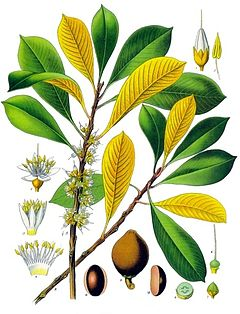
\includegraphics[width=0.50000\textwidth]{Sapotaceae.jpg}
\caption{hojas, flores y fruto de la familia Sapotaceae\label{imagen}}
\end{figure}

\begin{longtable}[]{@{}lllll@{}}
\toprule
p1 & p2 & p3 & p4 & p5\tabularnewline
\midrule
\endhead
10 & 16 & 62 & 33 & 34\tabularnewline
20 & 15 & 22 & 32 & 32\tabularnewline
30 & 38 & 23 & 12 & 46\tabularnewline
\bottomrule
\end{longtable}

\section{Metodología}\label{metodologuxeda}

\ldots

\section{Resultados}\label{resultados}

En toda la parcela, se registró un total de 2029 pertenecientes a 5
especies. La riqueza por cuadro fue de 4 especies y la mediana de la
abundancia por cuadro fue de 39 individuos. La especie más abundante fue
\emph{Pouteria reticulata}, con 1084 individuos, y la menos abundante
fue \emph{Pouteria fossicola} con 3 individuos. La tabla
\ref{tab:abun_sp} y la figura \ref{fig:abun_sp_q} resume estos
resultados.

\begin{longtable}[]{@{}lr@{}}
\caption{\label{tab:abun_sp}Abundancia por especie de la familia
Sapotaceae}\tabularnewline
\toprule
Latin & n\tabularnewline
\midrule
\endfirsthead
\toprule
Latin & n\tabularnewline
\midrule
\endhead
Pouteria reticulata & 1084\tabularnewline
Chrysophyllum argenteum & 711\tabularnewline
Chrysophyllum cainito & 171\tabularnewline
Pouteria stipitata & 60\tabularnewline
Pouteria fossicola & 3\tabularnewline
\bottomrule
\end{longtable}

\begin{figure}
\centering
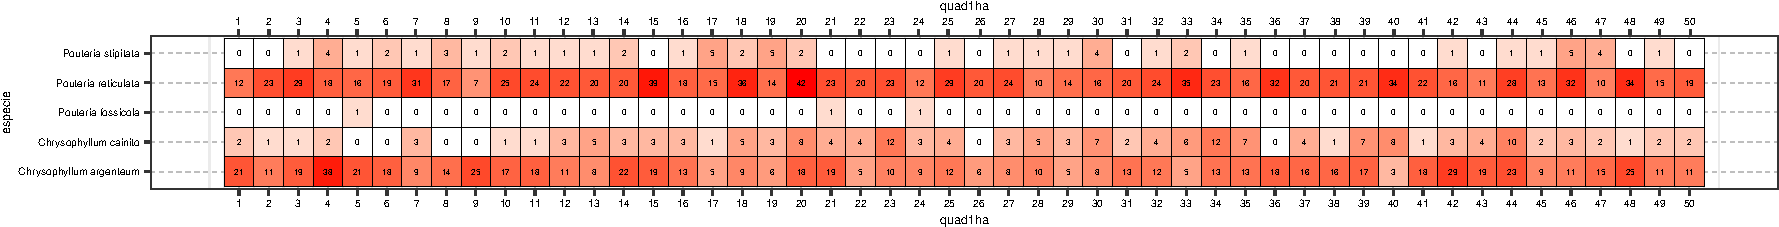
\includegraphics{manuscrito_files/figure-latex/unnamed-chunk-3-1.pdf}
\caption{\label{fig:abun_sp_q}Abundancia por especie por quadrat}
\end{figure}

\begin{figure}
\centering
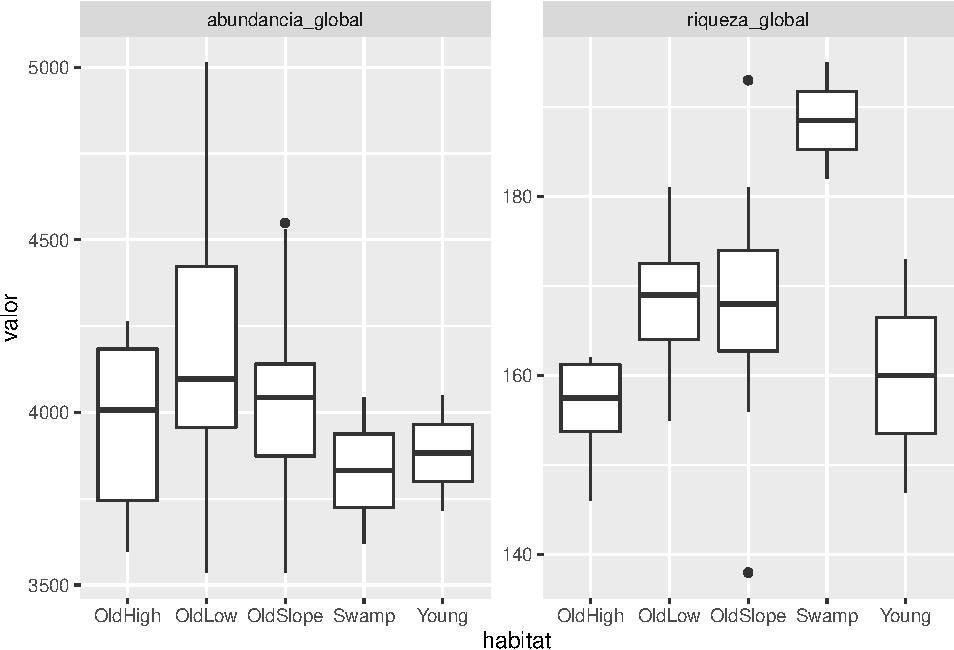
\includegraphics{manuscrito_files/figure-latex/unnamed-chunk-4-1.pdf}
\caption{\label{fig:P13}Diagrama de cajas de la abundancia y riqueza
segun habitats}
\end{figure}

la distribucion de la riqueza numerica de especies de la familia
Sapotaceae sigue un patron homogeneo, lo cual los agregados de riqueza
maxima estan distribuidos en casi todo el area. (ver Figura
\ref{fig:mapa_cuadros_riq_mi_familia})

\begin{figure}
\centering
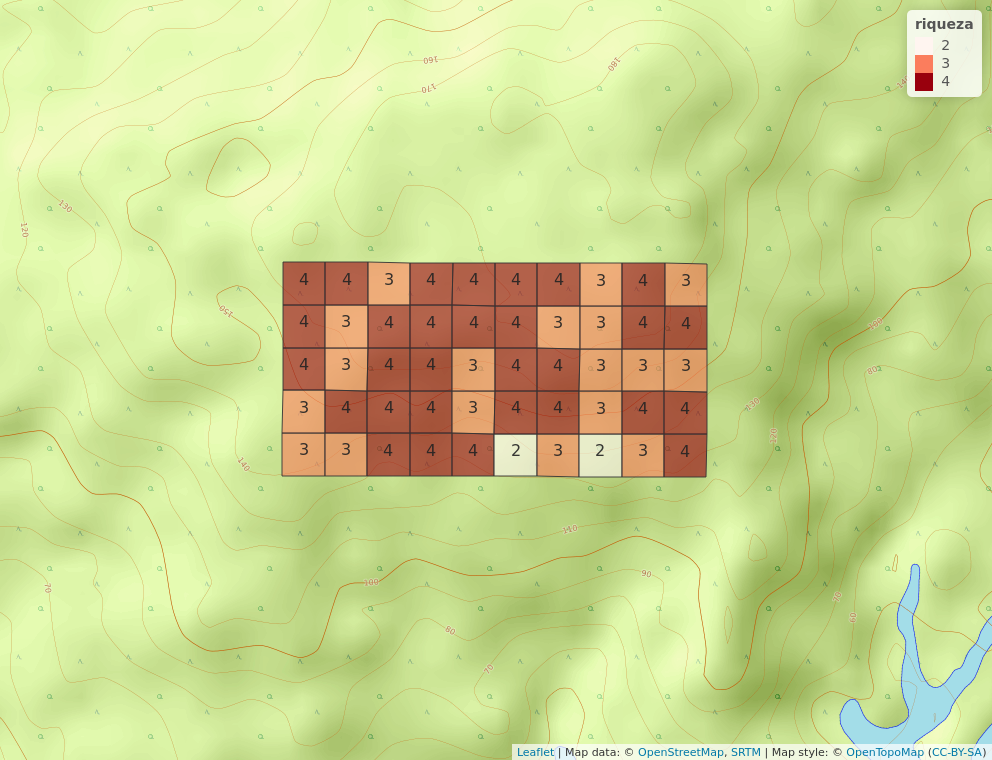
\includegraphics[width=0.50000\textwidth]{mapa_cuadros_riq_mi_familia.png}
\caption{Distribucion de la riqueza de la familia
Sapotaceae\label{fig:mapa_cuadros_riq_mi_familia}}
\end{figure}

Las variables ambientales pH y pendiente media presentaron asociacion
con la familia de plantas\ldots{}, lo cual supone\ldots{} (ver figuras
\ref{fig:mapa_cuadros_pH} y \ref{fig:mapa_cuadros_pendiente}).

\begin{figure}
\centering
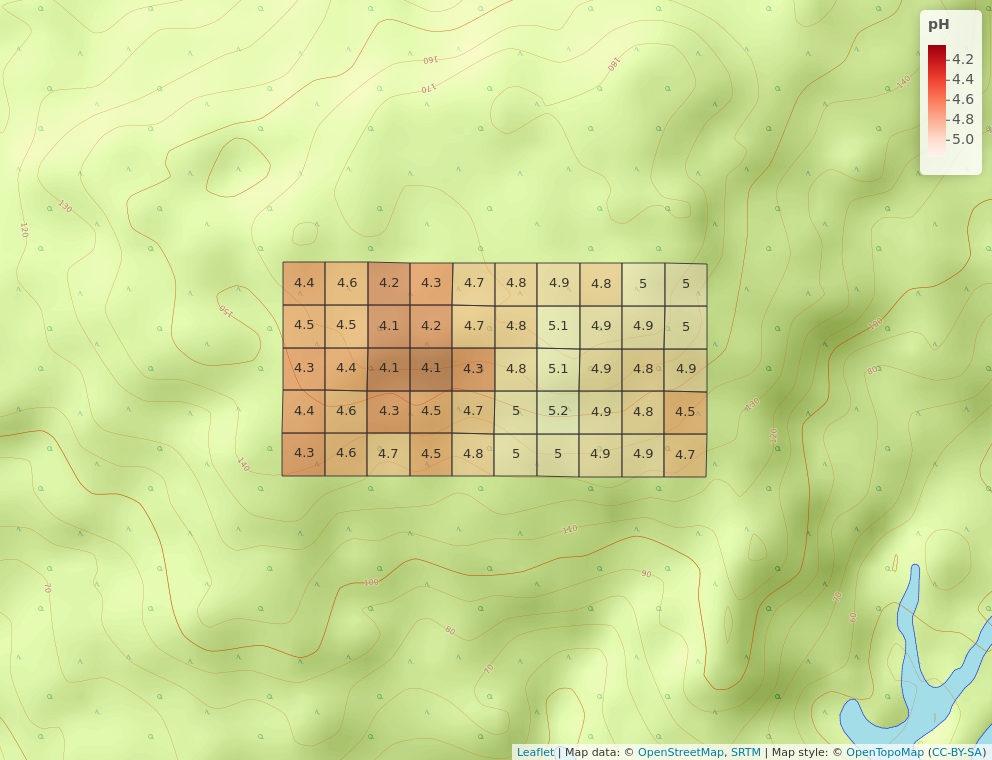
\includegraphics[width=0.50000\textwidth]{mapa_cuadros_ph.png}
\caption{Distribucion del pH\label{fig:mapa_cuadros_pH}}
\end{figure}

\begin{figure}
\centering
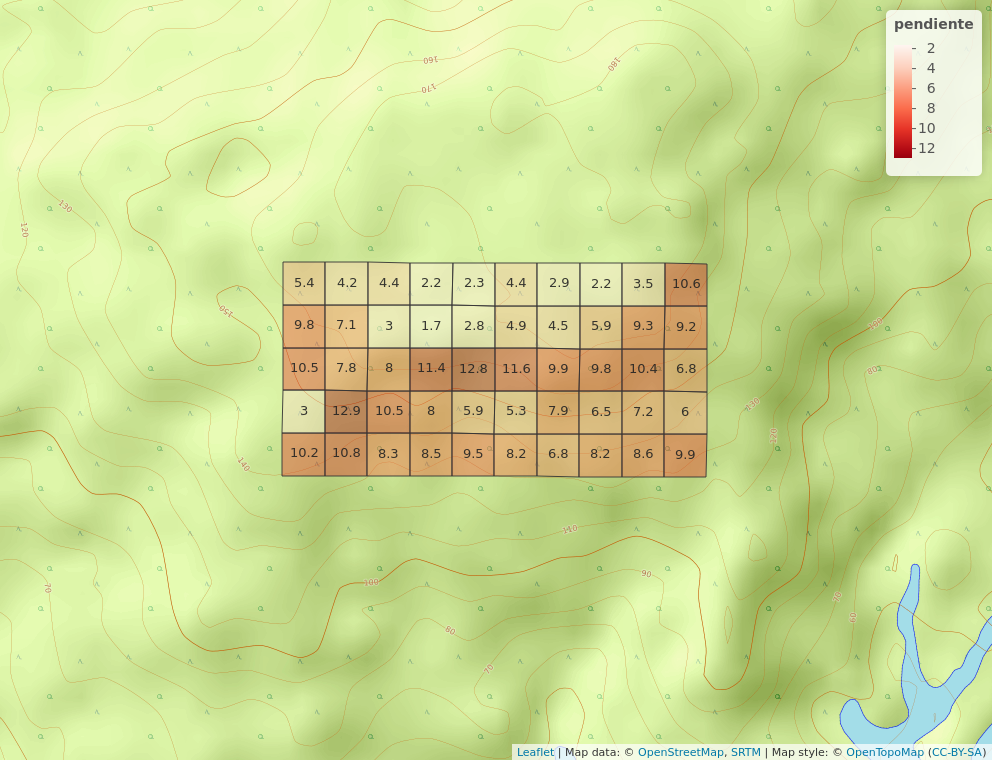
\includegraphics[width=0.50000\textwidth]{mapa_cuadros_pendiente.png}
\caption{Distribucion de las pendientes(en
grados)\label{fig:mapa_cuadros_pendiente}}
\end{figure}

la abundancia de la familia sapotaceae solo presenta correlacion con la
abundacia global, mientras que la riqueza tiene correlacion con la
presencia de cobre y nitrogeno en el suelo, lo que sugiere\ldots{} (ver
figura \ref{fig:p_cor_suelo_ar}).

\begin{figure}
\centering
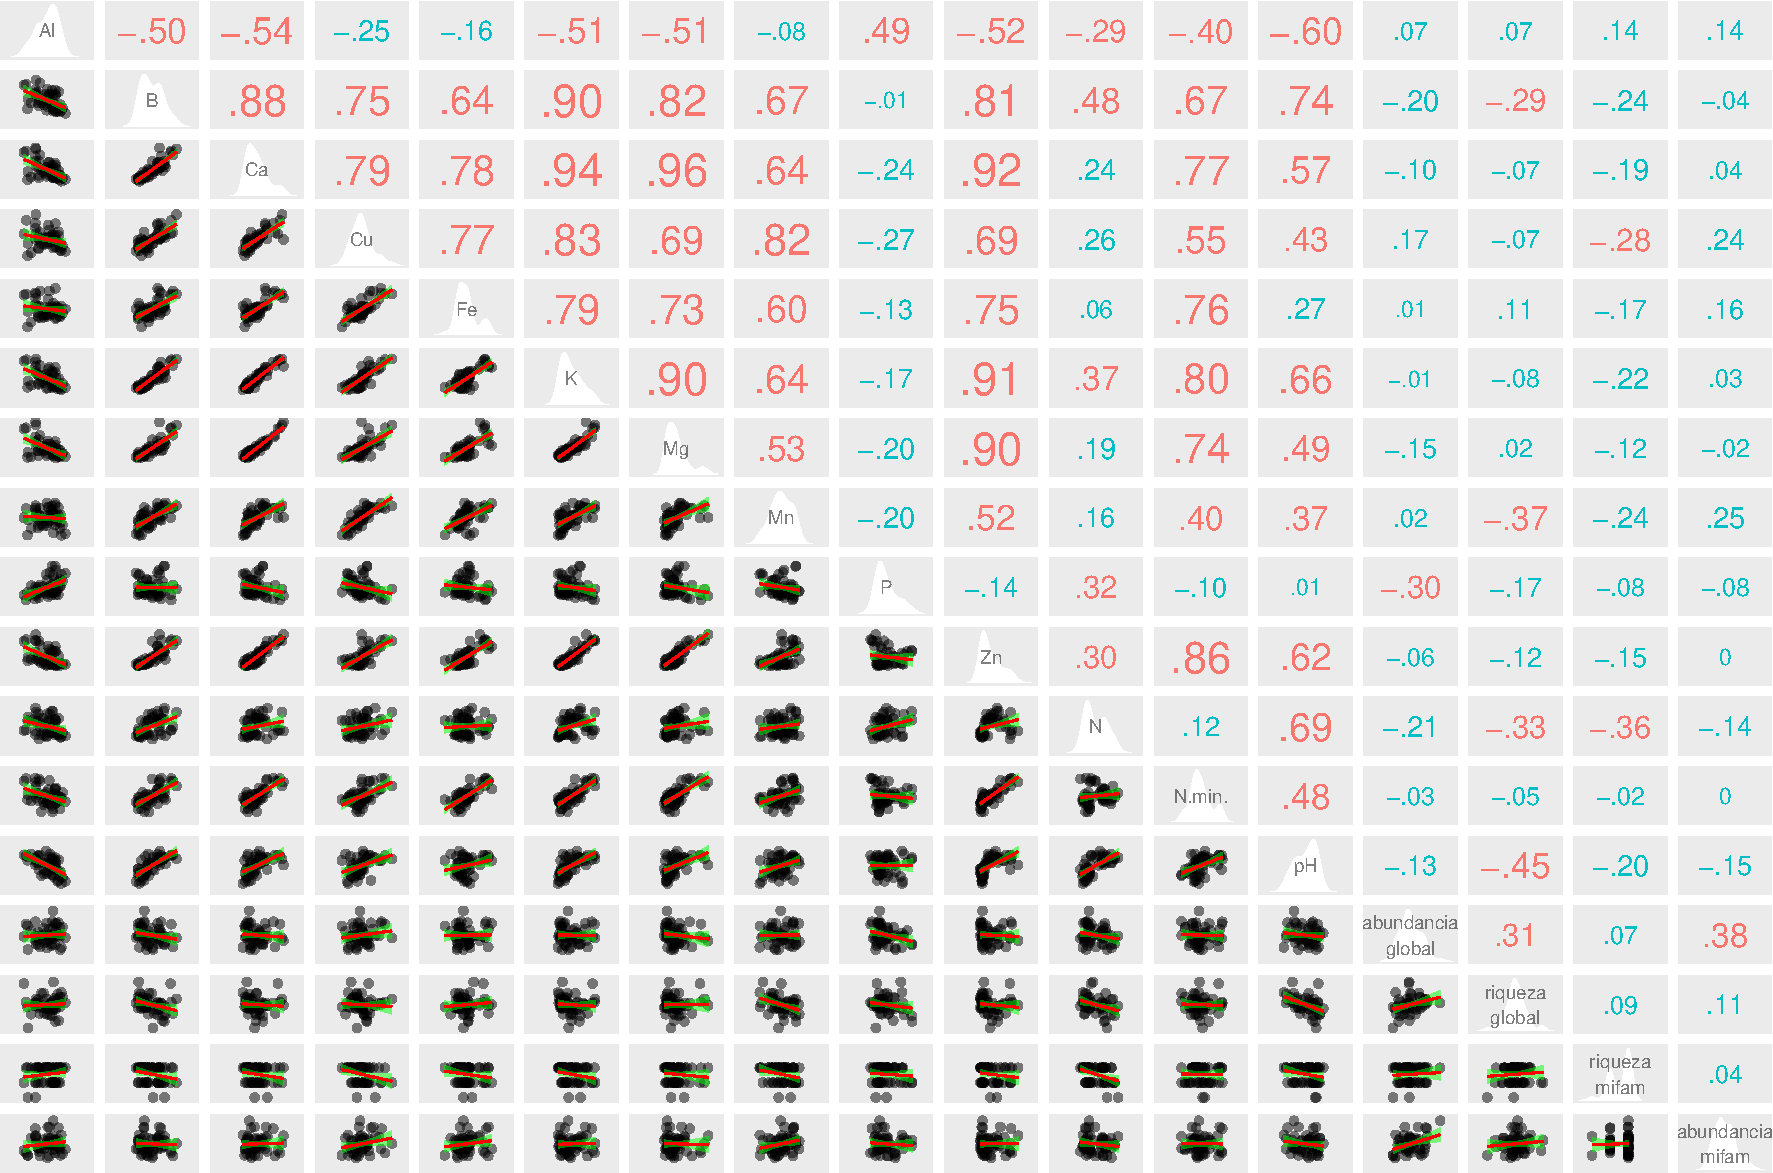
\includegraphics{manuscrito_files/figure-latex/unnamed-chunk-5-1.pdf}
\caption{\label{fig:p_cor_suelo_ar}correlacion de las variables del
suelo}
\end{figure}

las variables ambientales numericas y nominales presentan un
patron\ldots{} (ver figuras
\ref{fig:mapas_variables_ambientales_numericas} y
\ref{fig:mapas_variables_ambientales_nominales})

\begin{figure}
\centering
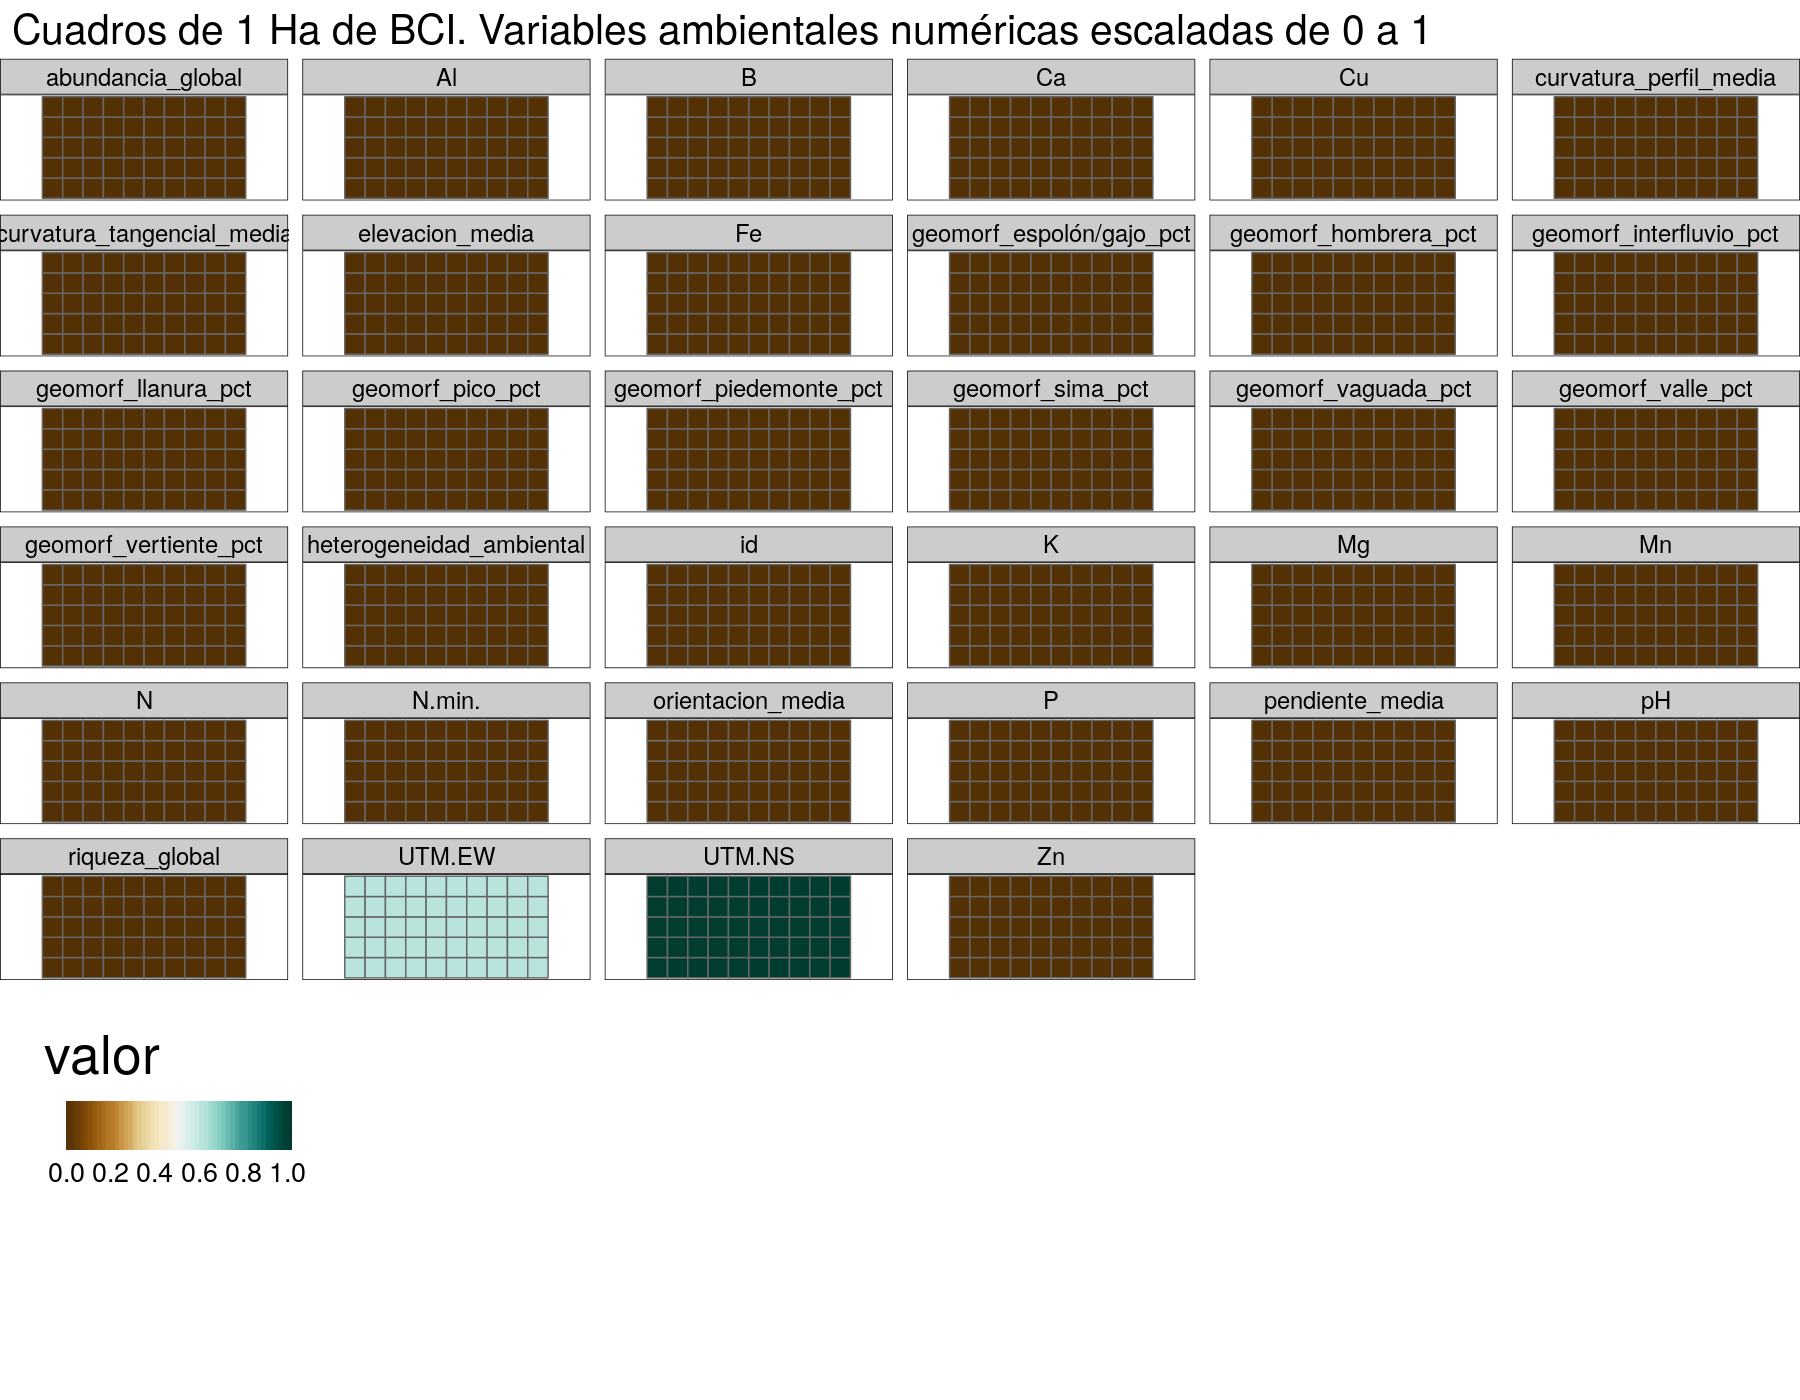
\includegraphics{mapas_variables_ambientales_numericas_tmap.png}
\caption{variables ambientales
numericas\label{fig:mapas_variables_ambientales_numericas}}
\end{figure}

\begin{figure}
\centering
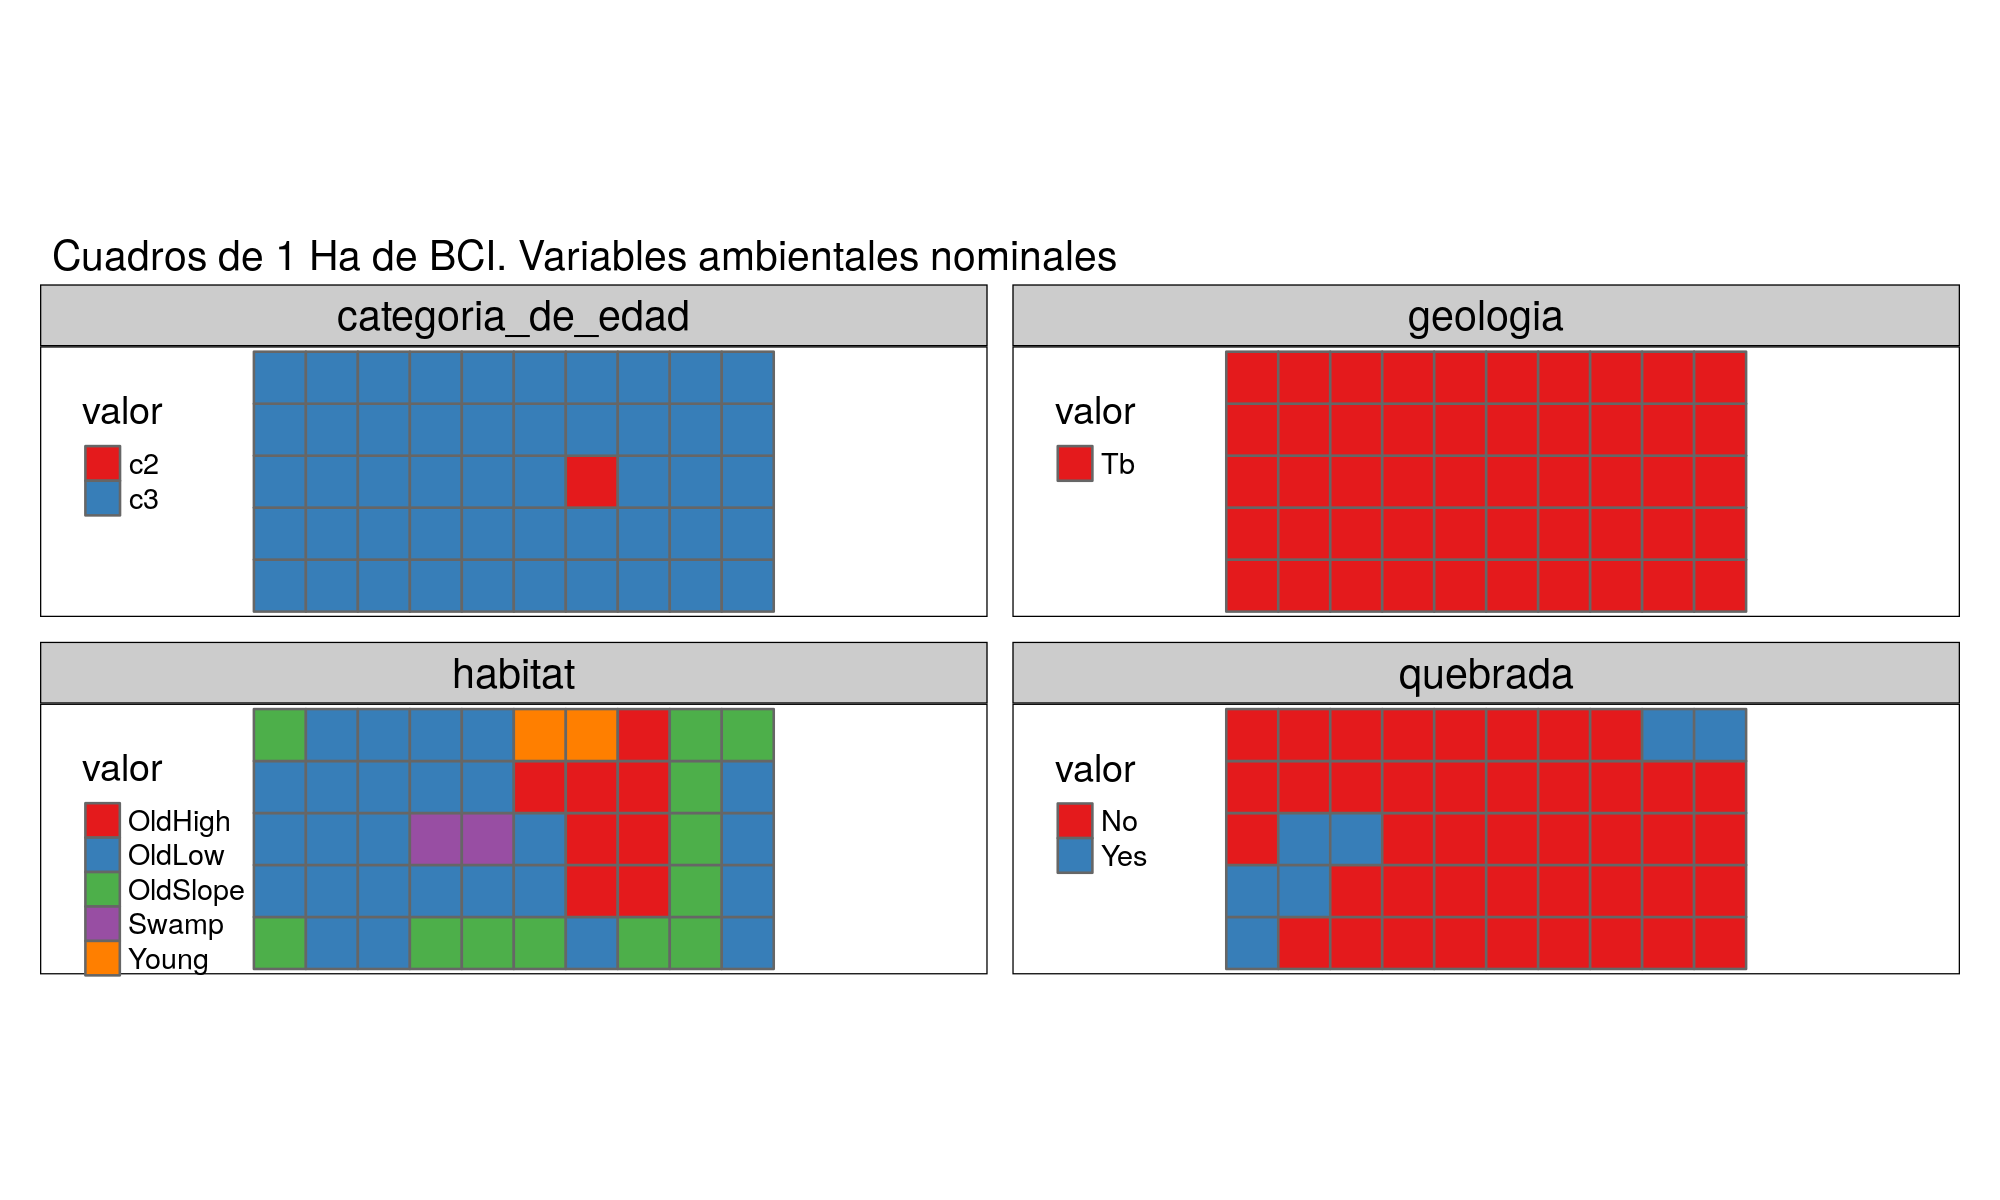
\includegraphics{mapas_variables_ambientales_nominales_tmap.png}
\caption{variables ambientales
nominales\label{fig:mapas_variables_ambientales_nominales}}
\end{figure}

\section{Discusión}\label{discusiuxf3n}

\section{Agradecimientos}\label{agradecimientos}

\section{Información de soporte}\label{informaciuxf3n-de-soporte}

\ldots

\section{\texorpdfstring{\emph{Script}
reproducible}{Script reproducible}}\label{script-reproducible}

\ldots

\section*{Referencias}\label{referencias}
\addcontentsline{toc}{section}{Referencias}

\hypertarget{refs}{}
\hypertarget{ref-henriquez2012fenologia}{}
Henríquez, C. A., Sotes, G. J., \& Bustamante, R. O. (2012). Fenología
reproductiva de pouteria splendens (sapotaceae). \emph{Gayana.
Botánica}, \emph{69}(2), 251--255.

\hypertarget{ref-martinez2020importancia}{}
Martínez-Sovero, G., Iglesias-Osores, S., \& Villena-Velásquez, J. J.
(2020). Importancia de la familia sapotaceae en madre de dios, perú.
\emph{Manglar}, \emph{17}(4), 287.




\newpage
\singlespacing 
\end{document}
